\section{Two-dimensional Колмогоров-Смирнов distance}

In order to check how different strategies approximate the toy-example distribution described in the next chapter, one had to settle for some kind of criterion. Because the general task is to approximate the integral 

$$ \expect f( X ) \text{  ,  } X \sim \pi$$

it is natural to settle for the Колмогоров-Смирнов distance, given by 

\begin{equation}\label{KS definition}
	\underset{x \in \real^\kk}{\sup} | F(x) - \hat{F}_\nn (x)|,
\end{equation}

where \Fecdf\, is the Empirical Cumulative Distribution Function, \ecdf , constructed from the chain generated by the \PT. 



The naturality of our criterion stems from the simple observation, that in practice we often forget that the whole \ecdf\, generated this way is a random measure, being extracted from a trajectory of the underlying stochastic process, and use it as a proxy for the real measure $\pi$. And so it seems natural to check for the distance expressed in equation \ref{KS definition}. 

ADD HERE THE VITALI SPACE

Suppose we are given a simulation with $\tilde{\nn}$ iterations after the burn-in period. It often happens that the algorithm stays for more than one iteration in certain sample points\footnote{In fact we can easily control the point sejour-time due to the random walk by manipulating the proposal step's distribution parameters. In case of the kernel generated by the conditional normal distribution, it suffices to diminish the entries of the covariance matrix.}. We count the occurences of that points and then normalise them dividing them by $\tilde{\nn}$ and call the result {\it a charge}. Thus, we are given a matrix with sample coordinates and their charges. If the target measure $\pi$ is absolutely continous with respect to the Lebesgue measure, then the points generated by accepted proposals should all differ on both of their coordinates, the measure of any submanifold of $\real^\kk$ being zero. If that is not the case, then we simply face the problem of computer's finite arithmetics and could solve it by a longer binary representation of the real numbers. In practice that is an extremely unlikely event and we will neglect it. Therefore we will from now on focus on points with distinct coordinates and refer to the number of thereof by $\nn$. The world {\it sample} will also be applied only to the uppermentioned points. 

The computations of the \KS might be computationally expensive, requiring, in pesimistic case, evaluation of the true Cumulative Distribution Function $F$ in approximately $\frac{\nn^\kk}{\kk!}$ points\footnote{The exact number being equal to number of points on the intersection of a $\kk+1$ dimensional simplex with the coordinates summing to $\nn$, and the $\mathbb{Z}^{\kk+1}$ lattice.}. To see that, let us focus in all of this section on the bivariate case\footnote{\dots the generalisation to higher dimension being straighforward.}.   


\begin{figure}
	\centering 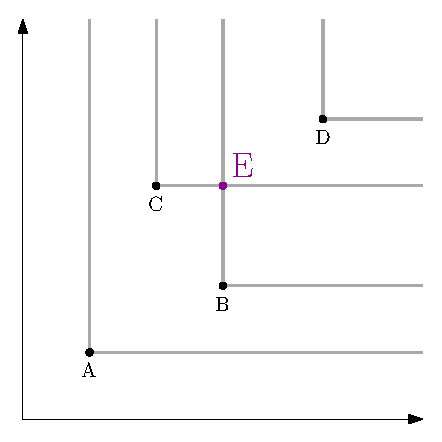
\includegraphics[scale=1]{./img/KS1.eps}
	\caption{Sample points and level sets of an examplary \ecdf.}\label{simpleEcdf}
\end{figure}


Observe, that the level sets of any \ecdf\, are uniquely determined by the sample points ( as $A, B, C$ and $D$ in Figure \ref{simpleEcdf} ) and points generated from them by taking the vectorised maximum

$$ 
	\begin{bmatrix} a_1 \cr a_2 \end{bmatrix} \vee 
	\begin{bmatrix} b_1 \cr b_2 \end{bmatrix} = 
	\begin{bmatrix} a_1 \vee b_1 \cr a_2 \vee b_2 \end{bmatrix},
$$ 
( such as $E$ in Figure \ref{simpleEcdf} ).  

One of the easiest way of establishing the values on the level sets of \Fecdf  is by considering a square, $(\nn+2)\times(\nn+2)$ matrix $B$, as in Figure \ref{spaceDivision}. The entries of $B$ correspond to values of \Fecdf\, on certain rectangles. Take the set of all $x$-coordinates of sample-points, $\Phi_x$, and the set of all $y$-coordinates of sample-points, $\Phi_y$. Add to them the coordinates of two dummy points: $(x_0, y_0)$ and $(x_{\nn+1}, y_{\nn+1})$ We enumerate points of these sets in the ascending order, $\Phi_x = \{ x_0 < x_1 < \dots <x_\nn < x_{\nn+1} \}$ and $\Phi_y = \{ y_0 < y_1 < \dots <y_\nn < y_{\nn+1} \}$. Then, the \Fecdf\, function is constant on rectangles 

$$R_{ij} = [x_i, x_{i+1})\times[y_j, y_{j+1}),$$ 
where $i,j \in \{0, 1, \dots, \nn+1 \}$. It is easy to realise now, that the number of level sets depends on the number of sample points and points generated by them using the vectorised maximum, $\hat{\nn} = \# \{ z : \exists x,y \in \text{Sample} x,y \not=z \text{ and } z = x \vee y \}$. This number is easily seen to be the greatest if all sample points could be arranged so that their $x$-coordinates strictly increase and $y$-coordinates strictly decrease.  

To actually derive the \KS\, we must assume that we can evaluate not only the true \cdf\, $F$, but also its two marginals\footnote{Limits of all the possible subsets of coordinates in infinity.}. Similarly to its univariate counterpart, the \KS\, can be calculated on only a finite number of points. Consider any rectangle. \Fecdf\, is constant on it. So the \KS depends solely on the evaluations of $F$ on that set. But $F$ is a distribuant - a function monotone in all its arguments, and so the maximum distance from \Fecdf\, can be attained only on the vertices of the rectangle. On the border rectangles ( $R_{i,\nn+1}$ and $R_{\nn+1,j}$ ) the evaluation simplifies to vertices adjacent to $R_{ij}$ rectangles and it is there, where we have to evaluate the marginals instead of $F$. \Fecdf\, is equal to zero on rectangles on the southern and western extremities. Thus we put $B_{i0} = B_{0j} = 0$. 

\begin{figure}
	\centering 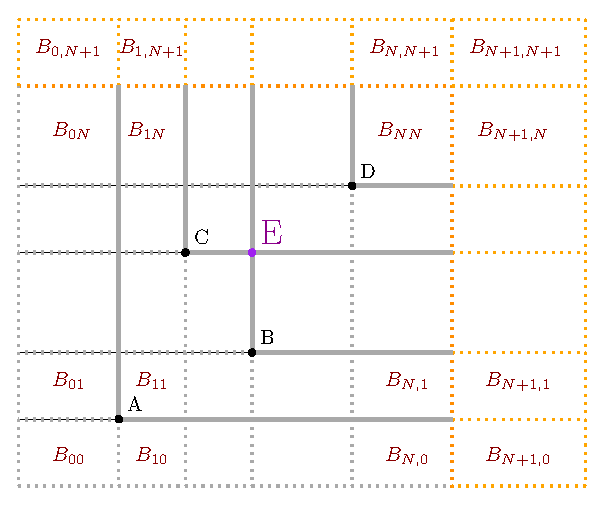
\includegraphics[scale=1]{./img/KS2.eps}
	\caption{How the $B$ matrix relates to the \ecdf level sets.}\label{spaceDivision}
\end{figure}


The rest of the algorithm is based on the dynamic programming approach introduced by \citet*{NiVingron} for comparing lists of changes in gene expression under different scoring regimes. The overall algorithm proceeds as follows:

\begin{minipage}[h]{\linewidth}
\begin{algorithm}
	\item Let $KS := 0$, $\jj = \nn+1$. 
	\item Read $\alpha$
	\item Prepare $\Phi_x$ and $\Phi_y$.
	\item While $i \in \{1, \dots, \nn+1\}$, and while $j \in \{ 1, \dots, \ii \}$ 
	\begin{algorithm}
		\item $B_{ij} := 
			\begin{cases} 
				B_{i-1,j-1} + \text{adequate charge}, \text{ if $R_{ij}$'s upper-left vertex is a sample-point} \cr
				B_{i,j-1} + B_{i-1,j} -  B_{i-1,j-1}, \text{ Otherwise} 
			\end{cases}$	

		\item\label{whenToEvaluate} If $i,j < \nn+1$ and both $B_{ij} > B_{i,j-1} \vee B_{i-1,j}$, then evaluate $F_{ij} = F(x_i, y_j)$.

		\item If either $i$ or $j$ equals $\nn+1$ evaluate the marginal distribtion.

		\item\label{changes} Evaluate $|F_{ij} - B_{ab}|$ at $a \in \{i-1,i\}$ and $b \in \{j-1,j\}$ or only on $i-1$ and $j-1$ if on border. If it is bigger than $KS$ then update $KS$. If the update occured and the new $KS$ is such, that $F_{ij}\wedge B_{ij} > 1 - KS - \alpha$ then update $\jj$ to $j-1$.

		\item Increase $j$ by one. After the end of loop increase $i$ by one.

	\end{algorithm}
	\item Return $KS$.
\end{algorithm}
\end{minipage}



Important changes with respect to \cite{NiVingron} can be seen in point \ref{changes} and the introduction of two extra variables $\jj$ and $\alpha$. The introduction of $\jj$ stems from the easy observation, that if both distribuant $F$ and \Fecdf\, are already in the interval $(1-KS,1]$, then any further evaluations of $KS$ to the East and North could not result in a bigger difference then the one already observed. Parameter $\alpha$ gives a further reduction in the number of calculations, enlarging that band to $(1-KS-\alpha,1]$, so that the true \KS will not be larger than by $\alpha$ from the value already established. We have also noted that it is not important to evaluate the real distribuant at every point of the matrix $B$. Rather than that, we note that because $F$ is a distribuant, evaluations are required on South-Eastern edges of the level sets, such as points $A, B, C, D$, and $E$ on Figure \ref{spaceDivision}. That is the reason behind point \ref{whenToEvaluate}. Other changes seem to be of minor importance and result from discretisation of the {\it a priori} continous problem. 


Our impelementation of the \KS calculator might not the optimal one. As pointed out by \citet*{Jon} the problem of calculating values of an \ecdf\, only in the sample points could be solved in $\mathcal{O}(\nn \log( \nn ))$ iterations. The existence of an algorithm requiring only $\mathcal{O}(\hat{\nn} \log( \hat{\nn}  ))$ operations, interesting in its own sake, will be object of further research.